\chapter{Statechart language}
\label{chap:runtime_verification}
We propose a statechart language as the modeling method used for the runtime verification of components. Many software is available for component generation or verification based on statecharts. Unfortunately the available solutions for verification and modeling provide limited syntax, and no error marking methods. Both leads to longer development, harder maintenance, and higher costs. The developed statechart language supports the verification of statecharts with parametric signals and timers, and enables the creation of template based statecharts that can be instantiated with parameters.
\section{Parametric statechart declarations}
The language allows a specification to consist of multiple statecharts. This feature led to of the main strength of the language: the definition of statechart templates, which can be instantiated parametrically. This results in ` descriptions for otherwise complex, but homogeneous systems with many similar components. Statecharts can be parametrized by values of well known data types. Separate statecharts can communicate with each other using signals or global variables.
\section{Parametric signals}
Signals can also be parametrized with integer type variables. These parameters can then be used to discriminate between similarly named signal raises, which results in more readable code, by allowing transitions to use the same signal as their trigger, when their functionality is similar.
\section{Overview}
For a brief overview of the basic capabilities of the language, see \cref{fig:verif}. The statechart describes a monitor for a round based game, where two players must press a button after the onStart signal was raised. The player who presses the button sooner wins. The game only ends after the second player has also made his move. The game enters a finish state and is restarted after 500 time units -- which is also the time between the beginning of the game and the first round. The system uses a local variable to determine which player won. In addition to this, the hardware has the capabilities to detect whether a button is stuck during the game phase. Should such occasion occur, the monitor enters a state called Stuck, which is marked as an error state.
\begin{figure}[H]
	\centering
	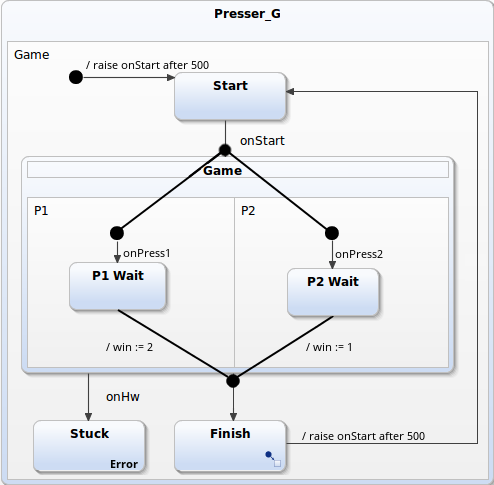
\includegraphics[width=0.65\linewidth]{include/figures/chapter_4/stcex}
	\caption{A simple statechart}
	\label{fig:verif}
\end{figure}

The description of the whole system is enclosed in a specification, which can have multiple statecharts, signals, and global variable declarations. Each statechart consists of a region and an optional number of local variable declarations. Regions encapsulate states and transitions. Each region must have at least an initial state. A state itself can have an arbitrary number of inner regions, which will run in parallel. States can also have entry and exit actions associated with them. Transitions must have a source and a target state, and optional triggers, guard conditions, and actions. States and transitions can be marked with an error token to indicate that the execution of the transition or the activation of the state is erroneous behaviour. Actions can be variable assignments and signal raises.

\section{Language syntax}
The language has a textual syntax that was designed to be simple without sacrificing expressiveness. The structure aims to be conform visual statechart languages, allowing one-to-one mapping where possible. Hierarchy is expressed by the scoping of elements. The naming of variables is similar to the conventions used by \verb!C!-style programming languages.
  \subsection{Specification}
Modelling the whole system as a single statechart would result in an overly complex statechart. Systems can usually be described as independent components that can communicate with each other. Therefore, an enclosing specification is used for the description of the whole system, within which statecharts can be declared as (mostly) independently operating components. Each specification can contain multiple statecharts. To enable communication between statecharts, global variable declarations and signal declarations are placed in the specification itself. For the model from \cref{fig:verif}, the specification of the system is:

\begin{lstlisting}
specification Game {
  signal onStart
  signal onPress1
  signal onPress2
  signal onHw
  statechart...
}
\end{lstlisting}

  \subsection{Statecharts}
  %TODO template magyaraz
The syntax for statechart definition would be in the form of:
\\\\\verb!statechart PushGame(!\textit{params}\verb!) {...}!\\\\
where \textit{params} is an optional parameter list, and \verb!{...}! contains the description of the statechart itself. The parenthesis can be omitted if no parameters were specified. Parametrized statecharts can be created from existing templates by providing a value for each parameter and omitting the description. Definitions without parameters are treated as an instantiation of the statechart. The system described by \cref{fig:verif} has no need for parameters, but should an integer type parameter be required, two statecharts could be instantiated as:

\begin{lstlisting}
statechart PushInstance1(1) := PushGame
statechart PushInstance2(2) := PushGame
\end{lstlisting}

A specification must contain at least one instantiated statechart.
  \subsection{Regions}
Statecharts are structured by the use of regions. At the root of every statechart, a region encloses all of the states. A state can have an arbitrary number of inner regions. This plays a fundamental part in the scoping of elements. A region can have both states and transitions. The syntax for a region is:
\\\\\verb!region Game {...}!\\\\
where the \verb!{...}! is the definition of the region's contents. Each region must contain at least an initial state for the model to be valid.
  \subsection{State nodes}
Regions can contain multiple state nodes. A state node can either be a state or a pseudo state. States create the base structure of the model, while pseudo states help to describe functionality. Pseudo states can either be initial-, fork-, join-, or choice states.

\cref{fig:verif} contains a composite state, three initial states, a composite state with two regions, and four simple states and an error state.

    \subsubsection{States}
States can either be atomic states or composite states. An atomic state is a state which does not contain inner regions. All states can contain entry and exit actions, which are executed when entering or exiting the state. Composite states contain one or more inner regions, each with at least an initial state. A state's parent state is it's containing region's containing state. If the region does not have a containing state, the parent is the region's containing statechart. Composite states allow users to maintain a clean model by the introduction of hierarchy, and the ability to describe common actions in the parent state.

These states could be described without the initial states and inner transitions as:

\begin{lstlisting}
state Start
state Finish
state Game {
  region P1 {
    ...
    state P1_Wait
    ...  
  }
  region P2 {
    ...
    state P2_Wait
    ...
  }
}
\end{lstlisting}

    \subsubsection{Initial states}
Initial states can be found in all regions - if the region's containing state is entered, these inner states become active. An example for an initial state as used in the first inner region of the Game state is:

\begin{lstlisting}
region P1 {
  initial state init
  ...  
}
\end{lstlisting}

    \subsubsection{Choice states}
Choice states are pseudo states whose outgoing transitions have exactly one of the guard conditions evaluating as true at all times. Choice states let the user create tree-like transition structures with simple guards conditions on each level, instead of rewriting similar, complex guard conditions using a single transition level. This usually results in more readable, modifiable, and expressive models. A choice state could be expressed as:

\begin{lstlisting}
choice whichPlayerWon
\end{lstlisting}

    \subsubsection{Fork and join states}
A fork state is a pseudo state that has a single incoming transition and any number of outgoing transitions. The outgoing transitions cannot have triggers, guards, or actions associated with them. If the incoming transition fires, all the outgoing transitions fire as well, and the fork state itself is not entered. This results in the simultaneous activation of multiple states.

A join state is a pseudo state that has a single outgoing transition and multiple incoming transitions. The incoming transitions cannot have triggers, guards, or actions associated with them. The outgoing transition is enabled when it's guard is true and all the incoming transitions' source states are active. Triggers can be declared on the outgoing transition.

The system from \cref{fig:verif} has both a fork and a join state. They can be expressed as:

\begin{lstlisting}
region Game {
  fork startSignalTriggered
  join allPlayersDone
  ...
}
\end{lstlisting}

  \subsection{Transitions}
Transitions describe the possible state changes. A transition can only occur if the source state is active. After the transition fires, the source state becomes inactive and the target state active. Furthermore, a transition can have a trigger, a guard condition, and an arbitrary number of actions associated with it. A simple transition is in the form of:

\begin{lstlisting}
region Game {
	...
	transition from Game to Start
	...
}
\end{lstlisting}

    \subsubsection{Transition triggers}
Transitions with triggers can only fire when one of the triggering signals arrive. Defining triggers is optional. Enabled transitions without a trigger occur on the next timestep after the source state becomes active. The transition to the error state in \cref{fig:verif} has a trigger, which can be expressed as follows:

\begin{lstlisting}
region Game {
	...
	transition from Game to Stuck on onHw
	...
}
\end{lstlisting}

    \subsubsection{Transition guards}
Transitions can have guard conditions, which are expressions that evaluate to a boolean value. If the guard condition evaluates to true, the transition is enabled, otherwise it is blocked. If we'd like to have transition that restarts the game when player one won, it would be (with no waiting):

\begin{lstlisting}
region Game {
	...
	transition from Finish to Start [win = 1]
	...
}
\end{lstlisting}

    \subsubsection{Transition actions}
A transition can have any number of actions associated with it. These actions are performed when the transition fires.

  \subsection{Actions}
Raising signals with or without a timeout, and variable assignments are called actions. They represent operations that might result in a change of the model's state.
  \subsubsection{Parametric signals}
Statecharts can communicate with the outside world and each other using signals. These signals are declared directly in the specification. Signals can be used with a single integer parameter (which can be either a constant or a variable). This allows much simpler syntax when dealing with communication, as a statechart can raise a signal and pass a value simultaneusly. It also leaves room for a later expansion to a token based automata with re-entry.
A parametric signal with the integer parameter 1 could be raised like:

\begin{lstlisting}
region Game {
	...
	transition from Finish to Start / raise onStart(1)
	...
}
\end{lstlisting}

where \textit{1} could be an integer-type variable declaration. A signal can be referenced multiple times, but only one transition may be taken per statechart for a raised signal. This results in a clearer model.
  \subsubsection{Timed signals}
Raising a signal can be offset by a certain amount of time. Apart from their delayed nature, timeout- and signal references can be used interchangeably. The starting timeout in \cref{fig:verif} can be raised by:

\begin{lstlisting}
region Game {
	...
	transition from init to Start / raise onStart after 500
	...
}
\end{lstlisting}

where \textit{500} is the number of timesteps before the signal is raised.
  \subsubsection{Variable assignments}
Variable assignments can be expressed with the syntax:

\begin{lstlisting}
region P1 {
	...
	transition from P1_Wait to forkState / assign win := 2
	...
}
\end{lstlisting}

An assignment's left hand side has to evaluate to an assignable reference, such as a variable or an array element. The right hand side can be any valid expression.
  \subsection{Timing of transitions and actions}
Transitions are fired one by one. The firing of a transition means that the triggering signal is consumed. This can result in non-deterministic runs if two transitions share the same trigger and can be enabled simultaneously. Such models can be created but should be avoided, as the order of the transitions is not guaranteed. Actions related to the current transition being taken are all executed in a single step.
  \subsection{Signaling errors, error propagation}
States and transitions can be labelled as errors. For states, the syntax is:

\begin{lstlisting}
region Game {
	...
	state [Error buttonStuck] Stuck
	...
}
\end{lstlisting}

For transitions, an example would be:

\begin{lstlisting}
region Game {
	...
	transition [Error buttonStuck] from Game to Stuck
	...
}
\end{lstlisting}

The \verb!buttonStuck! string is a description given by the user. This description is only used for the generation of error messages.
  \subsection{Expressions}
Variables can be used in expressions. Expressions can have an arbitrarily complex structure within the limits of the transition system described in \cite{fapts}. This allows the use of array indexing, parenthesis, and common operators in programming languages such as \verb!+!, \verb!-!, \verb!*!, \verb!/! --  just to mention a few. Assignments' left hand sides must reference a single variable while their right hand side is an expression. Logical expressions are also available (for example expressions using comparison operators). Each expression is a mixture of variables, constants, and operators. For a full reference, see \cite{fapts}.
  \subsection{Variables}
Variables can either be global (accessible to all statecharts) or local (bound to a single statechart in which they were declared). Many types are supported, like characters, integers, and doubles. For a complete list, see \cite{fapts}. Variable declarations are in the form of:

\begin{lstlisting}
statechart Game {
	local var win : integer
	...
}
\end{lstlisting}

where local (or global) denotes the scope of the variable of any of the supported types.
\section{Formal representation}
To enable formal verification of the defined systems, a mapping tool was developed that can generate transition systems (with the syntax described in \cite{fapts}) from statechart specifications. This means that complex concepts of the model have to be flattened out. The transition system used has the following major capabilities:
\begin{itemize}
  \item multiple independent transition systems can be defined
  \item these systems are enclosed in a specification
  \item transition systems can use local and global variables
  \item the state of a transition system can be defined as a vector of all referenced variables
  \item multiple states can be represented by expressions that restrict certain variables' values and leaves the rest of them unbound
  \item such restrictions are logical formulas with variables
  \item transition systems have transitions that represent changes of state using the referenced variables previous and current values
\end{itemize}
  \subsection{Specification}
The specification of the statechart language is mapped to the specification of the transition system. Global variables cannot be declared in the transition specification itself, they must be referenced in each transition system that uses them. Signals will be mapped to global variables.
  \subsection{Statecharts}
Each statechart is mapped to a separate transition system. These transition systems model systems running in parallel, which models the behaviour of the separate statecharts - they define systems that can communicate with each other but are running independently. Local variables in statecharts have the same local representation after mapped, and need no conversion.
  \subsection{Regions}
A transition system does not support hierarchical structures -- they are flat models. This means that all regions, states, and transitions inside a statechart are mapped directly into a transition system.
  \subsection{States}
States are represented as boolean variables that indicate whether a state is currently active or not. As entry and exit actions are unknown concepts in a transition system, these actions are propagated to all of the incoming and outgoing transitions of the state. This way any transition that would result in the entering or exiting of the state executes the appropriate actions.

Composite states entry and exit actions and their incoming and outgoing transitions are propagated to the atomic states inside them. This means that only atomic states are represented in the transition systems.
  \subsection{Transitions}
Transitions between states are transitions in the transition system too. For a transition to be enabled, guard conditions have to evaluate as \verb!TRUE! for the current state of the system, the source state has to be enabled (meaning that the source state's boolean variable is true), and the transition should have no trigger or the triggering signal's boolean variable has to be true (representing that it was raised). When the transition fires in the formal model:
\begin{enumerate}
  \item the exit actions,
  \item the actions associated with the transition,
  \item and the entry actions of the appropriate states occur.
\end{enumerate}
  \subsection{Signals}
Signals can be used for communication between statecharts. As such, each transition system that references a signal needs to be able to check whether the signal was raised. Therefore, in the formal model signals are represented as a set of global boolean variables. The variable is true if the signal has been raised since the previous timestep. As each statechart referencing the same signal might react to it by the firing of a transition triggered by the signal, a separate global boolean is used for each transition system. Since each signal can only trigger a single transition inside any given statechart, more complexer solutions are not needed. As signals are stored as booleans, the parameters are stored and can be referenced as global integer variables.
  \subsection{Timeouts}
Timeouts are signals that are raised with an offset in the time domain. Handling timeouts in a transition system is a well researched area \cite{dutertre2004timed}. A separate timing system is created as a transition system to generate simulate timesteps. The system has a variable that stores the current time and each signal has a helper variable that represents when the signal has to be raised next. If a timeout is set, the offset of the timeout is added to the current time and this value is assigned to the helper variable. The timing system has a constantly enabled transition which increments the current time if no timeout can occur. For each timeout a transition is defined that is enabled when the current time is equal to the time stored in the helper variable. When this transition happens, the signal is raised. The helper variables are set to -1 by default to prevent false signal raises based on timeouts.
  \subsection{Variables and expressions}
Variable types are the same as in the statechart model. Global variables remain global ones, and local variables that are declared inside statecharts are mapped to local variables inside systems. Expressions need no further flattening as the expression library used by the transition system language and the statechart language is the same.
  \subsection{Verification}
The verification of the mapped system is based on LTL or CTL expressions. These can be defined at the end of the mapped specification. By default, the non-reachability of error states and transitions are the only verified properties.

\chapter{Synthesis of monitors}
\label{chap:synthesis_monitor}
Current methods for statechart based code generation usually result in poor quality code. We propose a method for monitor generation based on the statechart language described in \vref{chap:runtime_verification}. Our approach was to generate easily readable, extensible, object oriented \verb!C++! code, that can run in environments with limited resources -- primarily embedded systems.
\section{Mapping of elements}
  \subsection{Specification}
A specification consists of separate statecharts. To simplifying their handling, a class was created called \verb!StatechartRegistry! that can automatically iterate through each statechart and update their state one timestep at a time. This class is also responsible for the initialization process of the monitor. The name of the class does not represent the whole specification as global variables and signals are handled by utility classes.
  \subsection{Statecharts}
Statecharts are represented as classes with lists of all their transitions, states, and currently active states. Local variables are mapped to global ones for unified usage. The statecharts' names are also stored for the error signaling process. Statecharts have functions for calculating their enabled transitions, taking enabled transitions, and maintaining the list of active states.
  \subsection{State nodes}
State nodes represent states, initial states, join states, and fork states. Their mapping highly depends on their type.
    \subsubsection{States}
Atomic or complex states are represented by named objects. All of these objects are derived from the \verb!State! class. This object represents a state that has no entry and exit actions. If a state has entry or exit actions, a child class is generated where the appropriate entry and exit actions are represented as overrides for the \verb!Entry()! or \verb!Exit()! function. Classes are instantiated using the states' fully qualified names.
    \subsubsection{Initial states}
Initial states are mapped to \verb!State! objects. This general class also has a boolean variable that is set to \verb!TRUE! for initial states.
    \subsubsection{Fork, join, and choice states}
Fork, join, and choice states are not represented in the monitoring object. These state nodes modify the behavior of transitions, and are handled when mapping transitions.
  \subsection{Transitions}
Transitions are represented as objects connecting two states. An instance of the generic \verb!Transition! class has an \verb!isEnabled()! function that always returns true, and an empty \verb!action()! function that simply returns. A null-initialized list reference is also present that can point to a list of states. The list itself is only created for fork and join states to minimize memory usage. The triggers of the transitions are handled in a separate mapper class and are play no role in the creation of transition objects.
    \subsubsection{Simple transitions}
Transitions without actions or guards can be instances of the generic \verb!Transition! class, while transitions with guard conditions or actions are it's children with overloaded functions. Simple transitions have one source and one target state specified when instantiating them.
    \subsubsection{Transitions of choice states}
Transitions from, and to choice states are handled by a statechart preprocessor that unfolds choices to simple transitions with the needed guard conditions to conserve functionality. The call to the preprocessor is the first step of the monitor generation.
    \subsubsection{Transitions of fork and join states}
Incoming and outgoing transitions of a fork state are mapped to a single transition with a target state reference of null. The fork's outgoing transitions are stored in the separate list of state references. A join state's transitions are also mapped to a single transition with a source state reference of null. The fork's incoming transitions are stored in the separate list of state references.
  \subsection{Signals}
Signals are represented as instances of the \verb!Signal! class, which is a class that describes a named object containing an integer value. Raising a signal means creating an instance with the appropriate name and parameter and putting it in a queue for processing in the next timestep. Signals with a timeout are stored in a separate row until they should be raised. Parameterless signals are signals with a parameter of a predefined, unused value.
  \subsection{Actions}
    \subsubsection{Raising signals and timeouts}
Signals can be raised by creating a signal object and placing it in the queue for arrived signals. Timeouts are signal raises that will occur in the future. When raising a timeout, the appropriate signal is created and put in a queue that holds pairs of signals and timestamps. The timestamp represents when the signal should go off.
    \subsubsection{Variables and expressions}
The assignments and expressions that can be used in the statechart language are a subset of the \verb!C++! language, so the mapping between the statechart language and the generated monitor adds no restrictions and require no extra constructs.
  \subsection{Variables}
The variable types of the statechart language are plain old data types in C++. Local variables are converted to global variables with fully qualified names. This allows a variable container class to be created which holds all of the variables and allows unified usage.
\section{Implementation}
The implementation of the monitoring component can raise many questions about timing issues. To generate working, and easily usable code additional helper classes and extra functions for the already described ones are required. As such, the most important utility classes are also described in this section.
  \subsection{Timing related issues}
The generated monitoring component will run on a real hardware. This means that the system can only take a limited number of transitions per second. Aiming for a lightweight component, there is a settable sleep and timeout period. The default implementation of the utility classes enables the user to set this period with millisecond precision.

For each timestep, the monitor:
\begin{enumerate}
  \item wakes up
  \item checks the future signals queue for elapsed signals
  \item puts such signals in the arrived signal's queue
  \item selects a statechart
  \item checks for transitions that can be fired
  \item fires one of them and apply the related actions
  \item updates the list of active states
  \item repeats from step 5 until no transition is enabled
  \item repeats from step 4 until no statechart is left
  \item goes to sleep for the set sleep period
\end{enumerate}
Raising signals while taking a transition puts the raised signal in a separate row that will be switched for the currently used one before going to sleep again. This means that only those transitions are taken whose triggers arrived in the queue before waking up. A signal with a timeout of \verb!x! means that the signal will be raised on the next awakening after \verb!x! milliseconds will have passed.
  \subsection{Utility classes}
A few utility classes are needed to keep the structure of the code more readable, or to make the functionality more customizable. The most important classes are listed under this section.
    \subsubsection{SignalRegistry}
A class called \verb!SignalRegistry! was introduced to create a thread-safe wrapper for signals, and a maintainer of signals with timeouts.
    \subsubsection{VariableRegistry}
All variables are treated as global variables. For availability and enclosure, we choose to create a centralized class with static variables resembling each variable found in the original statechart descriptions.
    \subsubsection{Timestamp}
For easily replaceable timing settings, the handling of timing properties is done by a separate \verb!Timestamp! class. The default implementation is to use millisecond-resolution functions and classes of \verb!std::chrono!.
  \subsection{Signal pushing}
The monitoring component starts in a separate thread. This means that calling the \verb!start! function will only block the current thread as long as the initialization process is running. After starting the monitor, the \verb!SignalRegistry::SignalArrived(!\textit{param}\verb!)! function can be called to inject a signal with the name \textit{param} into the system from the outside world. Naturally, the \verb!SignalRegistry! class is thread-safe.
  \subsection{Error signaling}
The \verb!OnError(!\textit{param}\verb!)! function is called upon reaching an error state or transition. The \textit{param} is equal to the specified message defined in the statechart model, or in case of states that have not defined a message, the fully qualified name of the error state. The function should be modified by the user to implement the necessary error signalling steps of the system.